\documentclass[10pt,journal]{IEEEtran}  %10pt, sans, memo

\usepackage{subcaption}
\usepackage{amsthm}

\usepackage[utf8]{inputenc}

\usepackage{tikz}
\usepackage{tikzscale}
\usepackage{pgfplots}

\usepackage{booktabs}
\usepackage{graphicx}
\usepackage{mathtools}
\usepackage{breqn}
\usepackage{natbib}

\usepackage{hyperref}

\bibliographystyle{ieeetr} 

\author{Jonathan Dyer}
\date{\today}
\title{Imaging Trends and the Future of Satellite Remote Sensing}
\hypersetup{
 pdfauthor={Jonathan Dyer},
 pdftitle={EO Modalities},
 pdfkeywords={},
 pdfsubject={},
 pdfcreator={}, 
 pdflang={English}}

\newcommand{\includepgf}[3]
{
  \begin{figure}[h!]
  \centering
  \includegraphics{#1}
  \caption[]{#3}
  \label{#2}
  \end{figure}
}
\DeclarePairedDelimiter{\abs}{\lvert}{\rvert}
\DeclarePairedDelimiter{\norm}{\lVert}{\rVert}

\begin{document}

\newtheorem{mydef}{Definition}

\makeatletter
\newcommand\footnoteref[1]{\protected@xdef\@thefnmark{\ref{#1}}\@footnotemark}
\makeatother

\author{Jonathan~Dyer,~\IEEEmembership{Member,~IEEE,}
        Dirk~Robinson,~\IEEEmembership{Member,~IEEE,}
        and~Paul~Boerner,~\IEEEmembership{Member,~IEEE}%
}

\markboth{Journal of \LaTeX\ Class Files,~Vol.~14, No.~8, August~2015}%
{}
        
        
\IEEEtitleabstractindextext{%
\begin{abstract}
The abstract goes here.
\end{abstract}


% Note that keywords are not normally used for peerreview papers.
\begin{IEEEkeywords}
IEEE, remote sensing, satellite, spacecraft, high resolution.
\end{IEEEkeywords}}

% make the title area
\maketitle

\IEEEdisplaynontitleabstractindextext

\section{Introduction}
\label{sec:introduction}

The last 15 years have seen a massive upheaval in digital imaging culminating in almost total obsolescence of film-based imaging.  Initially driven by the pro-sumer DSLR and pocket camera market, the trend has continued and accelerated with the introduction and refinement of high quality cameras in to smart phones and the digitization of the TV and Movie industries.

Satellite remote sensing systems underwent a similar revolution roughly 30 years earlier as film-based systems were phased out in favor of CCD-based electronic line scanners.  While the specific demanding requirements of satellite remote sensing drove much of the early technology investment and development in digital electronic imaging, far more investment is now being applied in the commercial arena than in further refinement of now mature CCD-based line scan sensors.

We assert that the future of the satellite remote-sensing industry will be in leveraging the massive investment in commercial digital and computational imaging technologies rather than continued large-scale investment in standalone technologies for these systems and that this shift presents both opportunities and challenges to new systems.

\section{Sensor Technology Trends}
\label{sec:sensor_trends}

Historically, space-based remotes sensing systems have utilized CCD-based Time Delayed Integration (TDI) line-scan sensors.  Modern TDI sensors are a mature technology with several very desire-able characteristics for high resolution remote sensing:

\begin{itemize}
    \item Purely electronic relative motion compensation through charge transfer
    \item High quantum efficiency and fill fractions
    \item Low noise
    \item Relatively high readout line-rates compatible with needs of high resolution systems
    \item Reasonable radiation tolerance
\end{itemize}

However the unique requirements associated with space-based sensors implies that the sensors are niche, low volume and typically very expensive to develop, integrate and use.

Meanwhile the large commercial investment in imaging sensors driven by the consumer photography and smart phone industries has resulted in incredibly high performance image sensors available at high volume and low cost.  The big trends that have developed due to this investment are:

\begin{itemize}
    \item Movement from CCD to CMOS detector technology
    \item Drive to smaller pixels to enable compact cameras
    \item Significant increase in detector read-out rates at low noise
\end{itemize}

CCD-based sensors still hold some performance advantages over CMOS sensors but the capability gap has narrowed almost entirely and the manufacturing and read-out rate advantages offered by CMOS have led to wholesale adoption.

When developing new remote sensing systems, the capabilities of modern commercial detectors promise the potential of smaller, less expensive systems with similar or better imaging performance to traditional TDI CCD-based systems.  However to realize this promise, the imaging system designer must consider the unique capabilities and shortcomings of the technology.

\section{Performance Trade Space}
\label{sec:trade_space}

The high resolution imaging trade space is fairly well constrained by a few driving requirements which are, in turn, driven by four primary mission needs:

\begin{enumerate}
\item Phenomenology
\item Image Quality
\item Collection Capacity
\item Cost
\end{enumerate}

\emph{Phenomenology} refers to the phenomenon being sensed or study and drives things like the spectral range, signal-to-noise ratio (SNR) and resolution required.  

\emph{Image Quality}, likewise, drives resolution and SNR.  

\emph{Collection capacity} drives many system variables both within the payload (such as swath width) as well as elsewhere in the spacecraft (collection rate, attitude control agility).  

\emph{Cost} is an increasingly important constraint placed on both technology selection and physical dimensions of the spacecraft.

We will largely ignore Phenomenology here and focus instead on the balance of Quality, Capacity and Cost in such systems.

\subsection{Remote Sensing Driving Requirements}
\label{sec:requirements}

Table \ref{table:drivers} shows the effect of many mission-level needs on lower-level requirements.
\begin{table}[h!t]
\resizebox{.45\textwidth}{!}{%
\begin{tabular}{@{}ll@{}}
\toprule
\textbf{Requirement} & \textbf{Drives} \\ \toprule
Resolution & \begin{tabular}[c]{@{}l@{}}Aperture Diameter\\ Altitude\\$Q$\end{tabular} \\ \midrule
\begin{tabular}[c]{@{}l@{}}SNR \& Dynamic Range\end{tabular} & \begin{tabular}[c]{@{}l@{}}Stabilization\\ Detector Full-well\\Optical $F^\#$\end{tabular} \\ \midrule
Swath Width & \begin{tabular}[c]{@{}l@{}}Optical Complexity\\ Detector Width\\ Data Volume\end{tabular} \\ \midrule
Collection Rate & \begin{tabular}[c]{@{}l@{}}Stabilization\\ Detector line-rate\end{tabular} \\ \midrule
Spectral Sampling & \begin{tabular}[c]{@{}l@{}}In-track FOV\\ Camera filters\\ Semiconductor Bandgap\end{tabular} \\ \bottomrule
\end{tabular}%
}
\centering
\caption{System Performance Drivers}
\label{table:drivers}
\end{table}

It is important to note that many of these requirements are tightly coupled.  %For example chosing a high resolution requirement directly impacts the difficulty of meeting other requirements:

%\begin{itemize}
%\item High resolution drives either a reduction in achievable SNR or a increase in required integration time and associated tighter ACS stability and more powerful image stabilization
%\item Recovering SNR at high resolution drives detectors with high line-rate (for digital oversampling) and/or significant analogy stabilization (TDI or optical)
%\item High resolution increases focal plane width and data intensity or reduces swath width while still increasing data intensity
%
%\end{itemize}

\subsection{Imaging Modalities}
\label{sec:modalities}

Digital imaging spacecraft have traditionally used a "push-broom" architecture where a line-array sensor is pushed along the ground by the spacecraft's motion.  Development of large format CCD and CMOS framing detectors allow for  "step-and-stare" architectures in which a scene snapshot is captured with a 2D framing sensor that is then moved further along the orbital path before another scene is captured.

\begin{figure}[hb!]
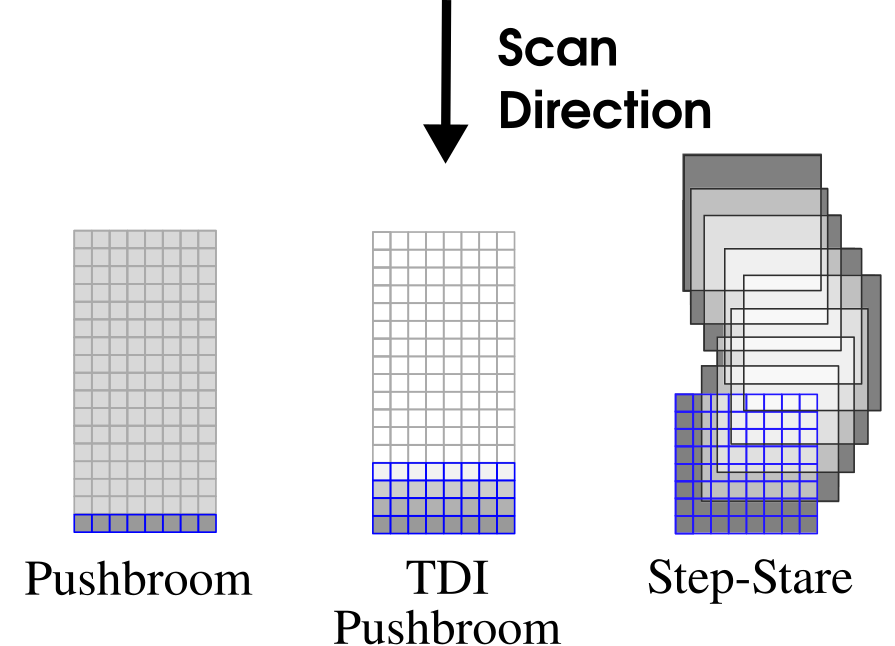
\includegraphics[width=0.42\textwidth]{figures/modalities.png}
\caption{General satellite imaging modalities}
\label{fig:modalities}
\end{figure}

Both TDI pushbroom and step-and-stare allow for some form of stabilization or motion compensation which is required to obtain reasonable $SNR$ in high resolution systems.  In the case of Figure \ref{fig:modalities}, analog charge transfer is depicted for TDI pushbroom and digital oversampling (through overlapping frames) is depicted for step-and-stare.  Pushbroom is shown mostly for historical reference as pure pushbroom collection is not feasible in systems with $GSD$ much below 10m.

\subsection{The case for smaller systems}
\label{sec:smaller}
The industry is in the midst of a shift toward smaller systems.  This is largely due to the cost, development speed and scaling advantages that constellations of small satellites offer.  Indeed \ref{bearden} has shown for historic small satellites that:

$$C \propto m^{1.261}$$

with a high correlation indicating that size alone is a major factor in system cost.

Happily, three trends in commercial image sensor and computing technology enable the development of smaller, lower cost spacecraft - 
\begin{itemize}
    \item Small pixels
    \item High read-out rates at low power
    \item High performance processing and storage at low power
    \item Inherent radiation tolerance of CMOS sensors
\end{itemize}

Other factors that are first-order influences on system cost which commercial imaging technologies positively impact are

\begin{itemize}
    \item Custom development cost and program risk
    \item Optomechanical components and integration
    \item Availability of development and test infrastructure
\end{itemize}

Before diving into these factors, we will define the different imaging modalities relevant to historical and future systems.


\subsection{Resolution and Pixel Size}

Resolution is a surprisingly difficult-to-define metric.  Often Ground Sample Distance (GSD) is used as a proxy for resolution under the assumption that all pixels are created equally.  This assumption doesn't hold for systems with widely varying SNR or sharpness (see Section \ref{sec:q}).

More holistic definitions of resolution typically refer back to \emph{resolvability} or the ability to distinguish objects or features of a given size in an image.  The so-called Ground Resolution Distance (GRD) is an example of a such a metric.  Unfortunately the definition of GRD is not universally agreed to or consistent.  We will use the definition of GRD proposed in \cite{auelmann_iq} where:

\begin{equation}
    \alpha_{eff} = \frac{IFOV}{RER} = \frac{\lambda_{mean}}{D_{ap} Q \times RER (Q)}
\label{eq:alpha_eff}
\end{equation}

\cite{auelmann_iq} has shown that a good approximation for $\alpha_{eff}$ for diffraction limited systems is given by:


\begin{equation}
    \alpha_{eff} \approx \frac{\lambda_{mean}}{D_{ap}}\left[1 + \frac{1}{Q^{1.35}}\right]^{1/1.35}
\label{eq:alpha_eff_approx}
\end{equation}

\includepgf{figures/resolution_q.pgf}{fig:resolution_q}{Relationship of GRD and GSD as resolution metrics as a function of Q}

Notice in Figure \ref{fig:resolution_q} that GRD asymptotes at $Q=2$ but that GSD continues decreasing monotonically.  This is because optical systems do not pass spatial frequency beyond the diffraction limit which is critically sampled at $Q=2$ and illustrates why GSD is a problematic resolution metric.

$Q$ is generally chosen as a trade between image quality, collection capacity and system size.  

[TODO: reference or discuss how collection capacity is impacted by Q]

More specifically, given a $Q$ and aperture diameter necessary to achieve mission image quality and collection capacity requirements, optical focal length and pixel size may be traded against each other directly.

$$Q \propto \frac{f}{p_{px}}$$

Historically because pixel sizes have been limited by CCD semiconductor process and well depth requirements (see ?? section) and swath width requirements would drive to unreasonably large focal planes at high $Q$, high resolution systems have been designed with $Q < 1$, leaving image quality on the table.  Even so, such systems typically have relatively high $F^{\#}$ ($> 10$) and thus focal lengths, $f$.  Both the pixel-size-driven focal plane sizes and focal-length-driven optical envelopes have been large and drive the rest of the system size.

$$m \approx s^3 \approx [f^3, p_{px}^3]$$

As we mentioned earlier, the recent emphasis is on smaller systems and, happily, the trend towards much smaller pixel in commercial image detectors opens up the opportunity.  However nothing comes for free and while the smaller pixels enable more compact systems, they also have smaller electron well depths and thus present a challenge in achieving acceptale $SNR$.  We will go into this further in TBD section and show how the digital and hybrid stabilized systems offer sa solution.

\subsection{Image Stabilization}

Large orbital velocity is a large advantage of spacecraft for remote sensing over other platforms as it gives:

\begin{itemize}
\item Daily global access
\item High collection rates
\end{itemize}

However it also presents large challenges in developing an imaging system that can collect sufficient light at the high relative scene velocity without incurring unreasonable blur.

For blur-limited integration times (unstabilized systems), in can be shown that \cite{shaw}

$$SNR \propto \frac{D_{ap} GSD^{3/2}}{\sqrt{V_{gnd}}}$$

Or if $SNR$ is a fixed requirement, relative ground velocity must be reduced such that:

\begin{equation}
V_{gnd} \propto GSD^3
\end{equation}

which has many system-level impacts, the largest of which is its impact on area collection rate, $ACR$:

$$ACR \propto GSD^4$$

This is a major challenge for high-resolution systems and historically there have been many solutions to compensate for scene motion on spacecraft.  These date back to the earliest film-based systems that used the film motion through the camera itself to compensate.  Other mechanical solutions included gimbaled cameras, "back-scan" of the entire spacecraft bus and full-aperture scan mirrors among others.

Indeed for systems with resolutions better than a few meters, some form of stabilization is essentially required to obtain sufficient $SNR$ without significant bus back-scan to reduce relative ground velocity.

We will classify modern stabilization strategies into three major buckets

\begin{enumerate}
\item Analog electronic charge transfer or time-delayed integration (TDI) stabilization
\item Digital oversampling stabilization
\item Analog optomechanical stabilization
\end{enumerate}

The analog techniques are considered such because they occur before digital sampling of the detectors and are thus still limited by detector well capacity.  Digital oversampling relies on detector line-rates high enough to enable multiple digital samples of a single ground point.

To-date analog electronic or TDI stabilization has only been implemented successfully in CCD detectors.  There is ongoing work to implement TDI in CMOS detectors but this technology is very immature - see \ref{sensor_tech}.  

Likewise digital oversampling is typically not practical using CCD sensors in high resolution systems due to the inherent limitations on read-out rate of CCD as compared with CMOS technology.

Analog optomechanical stabilization is implemented outside the detector such that it is potentially applicable to any sensor technology.

Finally it is important to point out that digital and analog stabilization can be combined in the same system.  Such hybrid stabilization schemes could be in the form of analog opto-mechanical stabilization plus digital oversampling or a TDI CCD that is read out fast enough to allow digital oversampling.  Indeed we will argue later that such hybrid stabilization schemes uniquely leverage the capabilities of modern CMOS detectors, enable smaller systems and provide significant system-level flexibility.

\section{Comparison of Modalities}
\label{sec:comp_modalities}

Table \ref{table:modalities} summarizes qualitatively the relative advantages and disadvantages of the three modalities with detailed analysis of each in the following sections.

\begin{table}[h!t]
\resizebox{.45\textwidth}{!}{%
\centering
\begin{tabular}{@{}rccccc@{}}
\multicolumn{1}{l}{}                                                 & \textbf{DR}                       & \textbf{SNR}                        & \textbf{Q \textgreater 1}         & \textbf{\begin{tabular}[c]{@{}c@{}}Stability\\ Req'd\end{tabular}} & \textbf{\begin{tabular}[c]{@{}c@{}}Data\\ Intensity\end{tabular}} \\ \cmidrule(l){2-6} 
\textbf{\begin{tabular}[c]{@{}r@{}}Analog \\Electronic\end{tabular}}                                                         & {\color[HTML]{F56B00} \textbf{-}} & {\color[HTML]{32CB00} \textbf{+}}   & {\color[HTML]{FE0000} \textbf{-}} & {\color[HTML]{FE0000} \textbf{- -}}                                & {\color[HTML]{32CB00} \textbf{++}}                                \\ \midrule
\textbf{\begin{tabular}[c]{@{}r@{}}Digital\\Oversampling\end{tabular}}                                                  & {\color[HTML]{32CB00} \textbf{+}} & {\color[HTML]{FE0000} \textbf{- -}} & {\color[HTML]{FE0000} \textbf{-}} & {\color[HTML]{32CB00} \textbf{++}}                                 & {\color[HTML]{FE0000} \textbf{- -}}                               \\ \midrule
\textbf{Hybrid} & {\color[HTML]{32CB00} \textbf{+}} & {\color[HTML]{32CB00} \textbf{++}}  & {\color[HTML]{32CB00} \textbf{+}} & {\color[HTML]{32CB00} \textbf{Tunable}}                            & {\color[HTML]{32CB00} \textbf{Tunable}}                           \\ \bottomrule
\end{tabular}%
}
\caption{Relative advantages, disadvantages of the modalities. $DR$ is dynamic range, $SNR$ is signal-to-noise ratio}
\label{table:modalities}
\end{table}
\subsubsection{High Dynamic Range Imaging}
\label{sec:hdr}

\section{Conclusions}
\label{sec:conclusions}

\section{Appendix A: Definitions}
\label{sec:appendix_a}

\subsection{$\frac{\lambda F^\#}{p}$ or Q}
\label{sec:q}

The system parameter $Q$ is defined as:

\begin{equation}
Q = \frac{\lambda F^\#}{p}
\label{eq:Q}
\end{equation}
and is essentially a measure pixel sampling in the spatial domain relative to the Nyquist criterion.  Nyquist says that to completely reconstruct a band-limited system, the spatial sampling frequency. 
$$\rho_s = 1/p \geq 2 BW_{opt}$$

Because we always sample to DC, the optical bandwidth $BW_{opt}$ is replaced by the diffraction cutoff frequency.
$$\rho_c = \frac{1}{\lambda F^\#}$$

Thus $Q$ is a measure of Nyquist sampling where $Q=2$ is critically sampled.  Most systems, however, operate at $Q < 2$ and hence incur some spatial aliasing.  There is little reason to operate at $Q > 2$ as the optics do not pass spatial frequency information there so the additional sampling is essentially wasted.

\begin{figure}[h!]
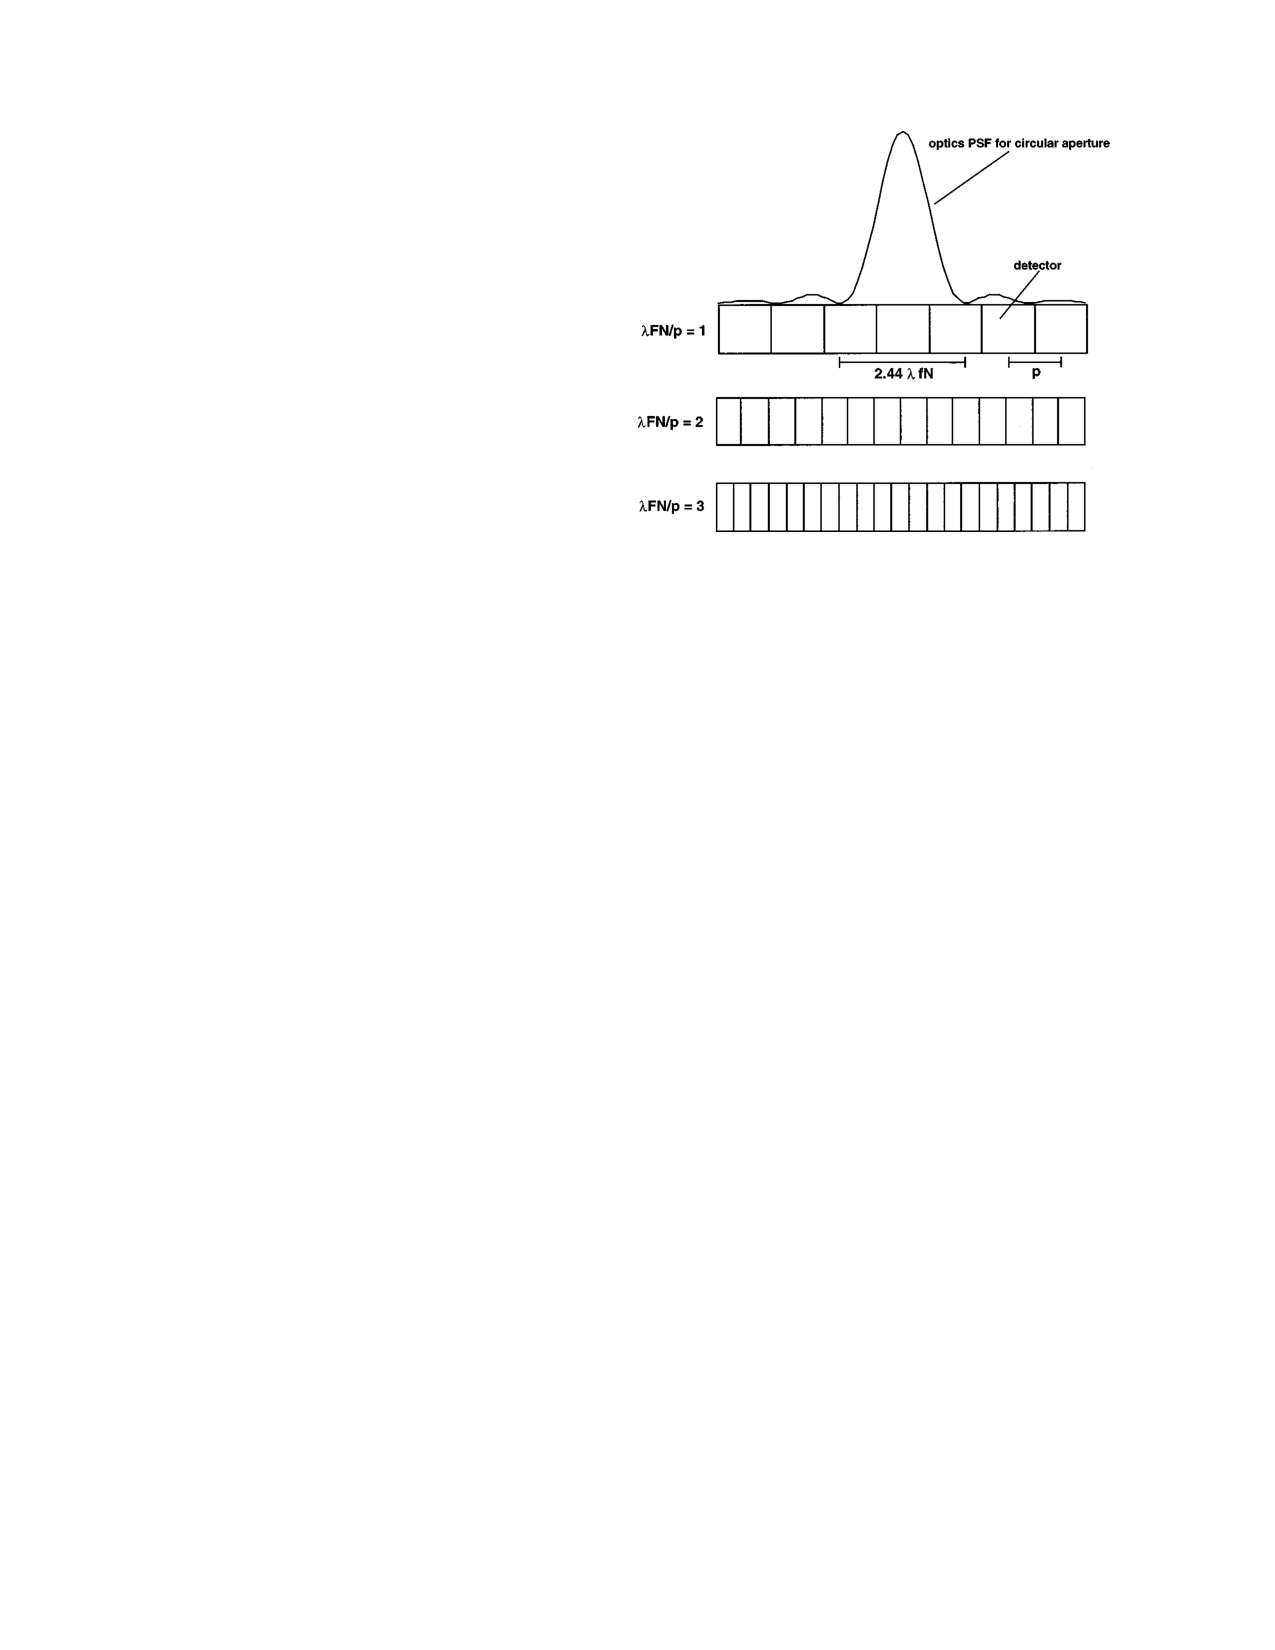
\includegraphics[width=0.42\textwidth]{figures/Q_fiete.pdf}
\caption{Spatial interpretation of Q sampling a diffraction-limited PSF.  Adapted from \cite{fiete_q})}
\end{figure} 

Beyond a statement of the Nyquist criterion, $Q$ is a very useful parameter by which to evaluate and compare systems.  For more see \cite{fiete_q}.  

\subsection{Image Quality}
\label{sec:iq}

Image quality is a complex, multi-faceted subject and while there is no perfect model or metric, substantial work has gone into quantifying the image quality of high resolution remote sensing systems.  Before jumping into integrated image quality models, we will define the geometric and radiometric components of image quality.

\subsubsection{NIIRS and GIQE}
High resolution systems are typically evaluated by quantitative "image interpretability" scales the best known being the National Image Interpretability Rating Scale, or NIIRS.

NIIRS rating is described by specific human interpretation standards, examples of which are shown in Table \ref{table:NIIRS}\cite{niirs}.

\begin{table}[h!t]
\resizebox{.45\textwidth}{!}{%
\begin{tabular}{@{}lll@{}}
\toprule
\textbf{NIIRS} & \textbf{GRD}          & \textbf{Description}                                                                                                                             \\ \toprule
3     & 2.5m - 4.5m  & \begin{tabular}[c]{@{}l@{}}Identify a road as divided or undivided\\ Detect rows of automobiles in a parking lot\end{tabular}           \\ \midrule
4     & 1.2m - 2.5m  & \begin{tabular}[c]{@{}l@{}}Detect barriers/obstacles (barrels) on runways\\ Distinguish between locomotives and railcars\end{tabular}   \\ \midrule
5     & 0.75m - 1.2m & \begin{tabular}[c]{@{}l@{}}Identify individual lines painted on paved roads,  parking lots\\ Identify fallen utility poles\end{tabular} \\ \midrule
6     & 0.4m - 0.75m & \begin{tabular}[c]{@{}l@{}}Detect individuals, when not in a group\\ Detect small road signs in an urban area\end{tabular}              \\ \bottomrule
\end{tabular}%
}
\centering
\caption{NIIRS definitions}
\label{table:NIIRS}
\end{table}

NIIRS is a logarithmic scale traditionally evaluated by trained human image interpreters.  However, much work has gone into developing semi-analytic regressions to predict NIIRS from basic image quality parameters such as sharpness, signal-to-noise ratio (SNR), etc. The Generalized Image Quality Equation (GIQE) is an example of such a function; we will use the 5th version, GIQE-5 which is defined in eq. \ref{eq:giqe5}.

\begin{dmath}
NIIRS = 4.4 - 3.32 \log(GSD_{m}) + 3.32 \left[1 - e^{\frac{-5.308}{\Delta SNR}}\right]\log(RER_0)
- 0.402 \log(RER_0)^4 - 2.92/\Delta SNR - 0.069N_{smear}
\label{eq:giqe5}
\end{dmath}
where $GSD_{m}$\footnote{GSD units must be paid close attention to - many references list GIQE using units of inches for GSD.  In this case, the first parameter in the equation is 9.7 rather than 4.4 because $4.4 - 3.32\log{\left(39.4 \frac{in}{m}\right)} \approx 9.7$} is the ground sample distance in meters, $\Delta SNR$ is difference between $SNR$ for a 15\% and 8\% target reflectance, $RER_0$ is the raw Relative Edge Response (without sharpening or MTFC) and $N_{smear}$ is the number of pixels of linear smear.

GIQE-5 is fairly well validated again human interpreters \cite{giqe5} and nicely captures the trade-off between various imaging system parameters such as $SNR$ and $GSD$.  

\includepgf{figures/Q_iq.pgf}{fig:q_iq}{Parametric study of GIQE-5 shows how optimal image quality depends on Q.  Note that this plot assumes $RER_0 = 0.3$ and $GSD = 1m$ for $Q=1$ and that $SNR \approx 1 / Q$}

One thing noticed in parametric study of the GIQE-5 is that image quality is often maximized at $Q>1$ (Fig. \ref{fig:q_iq}).  This has also been validated in human-interpreter studies \cite{fiete_Q_IQ}.

\subsubsection{Dynamic Range ($DR$) and Signal-to-noise Ratio ($SNR$)}
Dynamic range and signal-to-noise ratio are closely related by subtly different measures of radiometric performance.

Dynamic range is defined as the ratio of maximum-to-minimum signal level that the system can capture or represent in an image:

$$DR = \frac{S_{max}}{S_{min}}$$

The minimum signal level is the noise-floor of the system, $s_{min} = \sigma$ where $\sigma$ represents all non-signal-correlated noise sources in the system including read noise, dark current, etc.

The maximum signal is the maximum number of photo-electrons the system can capture for one output image pixel and is limited by the well depth of a pixel, $s_{max} = N_{e^-}^{well}$ for single-exposure systems.  Note that in digitally oversampled systems (covered later), the digital oversampling factor directlye expands dynamic range by increasing the effective well depth such that $s_{max} = N_f N_{e^-}^{well}$ where $N_f$ is the oversampling ratio.  Oversampling also affects $s_{min}$ and it can be shown that, for equally exposed samples:

\begin{equation}
    DR = \sqrt{N_f}\frac{N_{e^-}^{well}}{\sigma_{uncor}}
\label{eq:DR_OS}
\end{equation}

For systems that digitally oversample with unequal exposures, the dynamic range can be even larger as is shown in section \ref{sec:hdr}.

Signal-to-noise ratio, $SNR$, like dynamic range depends critically on both the detector well depth and its noise characteristics.  However signal-to-noise ratio is not purely a system-defined metric but depends also on the scene being imaged and as well as exposure parameters.  In general $SNR$ is defined as:

$$SNR = \frac{s}{\sigma_{noise}}$$

In general noise consists of the same sources discussed for $DR$ but also the shot-noise associated with the signal, $s$.  Because arrival rate of incoming photons obey Poisson statistics, it can be shown that $\sigma_{shot} = \sqrt{s}$ such that:

$$SNR = \frac{s}{\sqrt{\sum{\sigma_i^2} + s}}$$

In order to state an $SNR$, the signal, $s$, must be constrained by other system parameters and some exposure.  Typically $SNR$ is specified with respect to a specific target reflectance or top-of-atmosphere (TOA) radiance and a maximum or saturation reflectance or TOA radiance.  For a perfectly exposed scene with

$$\alpha = \frac{L_{typ}^\lambda}{L_{sat}^\lambda}$$
,
$$SNR_{\alpha} = \frac{\alpha N_{e^-}^{well}}{\sqrt{\sum{\sigma_i^2} + \alpha N_{e^-}^{well}}}$$

where $\alpha$ is the ratio of target radiance (or reflectance) to the saturation value.  This relation, like $DR$, can be expanded to include multiple digital exposures such that

\begin{equation}
\label{eq:snr_alpha_multiframe}
SNR_{\alpha} = \sqrt{N_f}\frac{\alpha N_{e^-}^{well}}{\sqrt{\sum{\sigma_i^2} + \alpha N_{e^-}^{well}}}
\end{equation}

For most modern detectors, uncorrelated noise sources are small compared with shot noise so we can approximate eq. \ref{eq:snr_alpha_multiframe}

\begin{equation}
\label{eq:snr_alpha_multiframe_simp}
SNR_{\alpha} \approx \sqrt{N_f \alpha N_{e^-}^{well}}
\end{equation}

\subsection{Collection Capacity}
\label{sec:capacity}
For a spacecraft, system collection capacity is constrained by a delicate balance between image collection capacity and the ability to get the collected data to the ground.  The latter is dictated entirely by data intensity, $I_D$, and communications bandwidth (which we won't go into here).  

Image collection capacity in turn depends on a number of parameters including ACS agility, swath width and imaging relative ground speed, $V_{gnd}$.  We will not discuss ACS agility here as it is not strictly an imaging system parameter but instead will parametrize it along with other factors such as time-in-sun into a single imaging duty-cycle, $\beta = \frac{t_{img}}{t_{per}}$ metric where $t_{per}$ is the spacecraft orbital period and $t_{img}$ is the imaging time per orbit.  

For remote sensing systems constrained by sun and time-over-land, typically $\beta < 0.1$.

There are two primary capacity regimes that a spacecraft may operate in:

\begin{enumerate}
\item Downlink-constrained regime
\item Collection-constrained regime
\end{enumerate}

In Regime 1:

$$t_{d/l} \times BW_{d/l} < I_D t_{per} \beta \frac{V_{gnd}w_{ct}}{GSD^2}$$

where $w_{ct}$ is the swath width or cross-track field of view projected to the ground, $t_{D/L}$ is downlink time per orbit and $BW_{D/L}$ is downlink bandwidth.  In Regime 2, the opposite holds.

We distill this down to a capacity constraint metric, $k_{cap}$

\begin{equation}
k_{cap} = \frac{t_{d/l}}{t_{per}} \frac{BW_{d/l} GSD^2}{I_D \beta V_{gnd} w_{ct}}
\end{equation}

We can now say that when $k_{cap} < 1$ the system is \emph{downlink constrained} and when $k_{cap} \geq 1$, the system is \emph{collection constrained}.


\subsubsection{Data Intensity}

Data intensity, $I_D$, is a metric that impacts a wide range of spacecraft subsystems from on-board storage and data handling to downlink bandwidth.  It is defined as the number of digital bits captured, processed or transmitted per image product output pixel

$$I_D \equiv \frac{N_{bit}}{N_{px}^{L1b}}$$

Where we assume an output product to consist of the fused, corrected but un-rectified L1b product. For a typical imaging pipeline that includes compression we must define exactly where in the system $N_{bit}$ is defined.  We will use the post-compression image data because it impacts the most system interfaces (storage, downlink, processing) and is generally directly proportional to the raw pixel data rate through the compression ratio, $C$

\begin{equation}
    \label{eq:compression}
    C \equiv \frac{N_{bpp}^{L0}}{N_{bpp}^{L1b}}
\end{equation}

For a digitally oversampling system

\begin{equation}
    I_D = N_f N_{bpp}^{L1b} = N_f C N_{bpp}^{L0}
\end{equation}

Note also that any resampling operations (including image reconstruction techniques such as super-resolution) impact $I_D$ since becaues for non-unity resampling ratios the number of output pixels is affected.  Thus we include a resampling factor

$${\eta}_{rs} = \frac{GSD_{L1b}^2}{GSD_{L0}^2}$$

such that

\begin{equation}
    I_D = {\eta}_{rs} N_f N_{bpp}^{L1b} = N_f C N_{bpp}^{L0}
\end{equation}

\subsection{Detector Line Rate}
For satelite remote sensing systems, the detector line rate, $LR$ is an important performance parameter because it limits the number of ground samples that can be captured.  For a push-broom system, $LR$ is simply defined as the number of in-track lines (or rows) that can be read from the detector per second:

$$LR = \frac{\Delta L}{\Delta t}$$

For a framing detector (reads out more than one in-track line per sampling period), we can define an equivalent $LR$ as
\begin{equation}
\label{eq:lr_framing}    
LR = \left(\frac{v_{pix}}{t_{frame}}\right)_{det}
\end{equation}

A necessary condition for the collection of contiguous, gapless imagery along the satellite's ground track is:

\begin{equation}
    LR \geq\frac{V_{gnd}}{GSD}
\end{equation}

where $V_{gnd}$ is the apparent velocity of the ground in the spacecraft's camera frame and $R$ is the range to the ground (equal to the spacecraft altitude when nadir-pointed).  This condition provides a lower-bound requirement on the detector line-rate at a given $GSD$.  

If $LR$ is high enough, it enables digital oversampling of a single ground location which has multiple potential uses that will be discussed in Section \ref{sec:step_stare}.  This has most relevance to framing detectors with significant in-track extent and we can define the oversampling ration, $N_f$:

\begin{equation}
    N_f = \text{floor}\left(\frac{GSD \times LR}{V_{gnd}}\right)
\end{equation}

\subsection{Entendue}
\label{sec:entendue}

\bibliography{main}

\end{document}
